\documentclass[tikz,border=2pt,png]{standalone}
\usepackage{tkz-euclide}
\usetkzobj{all}
\begin{document}
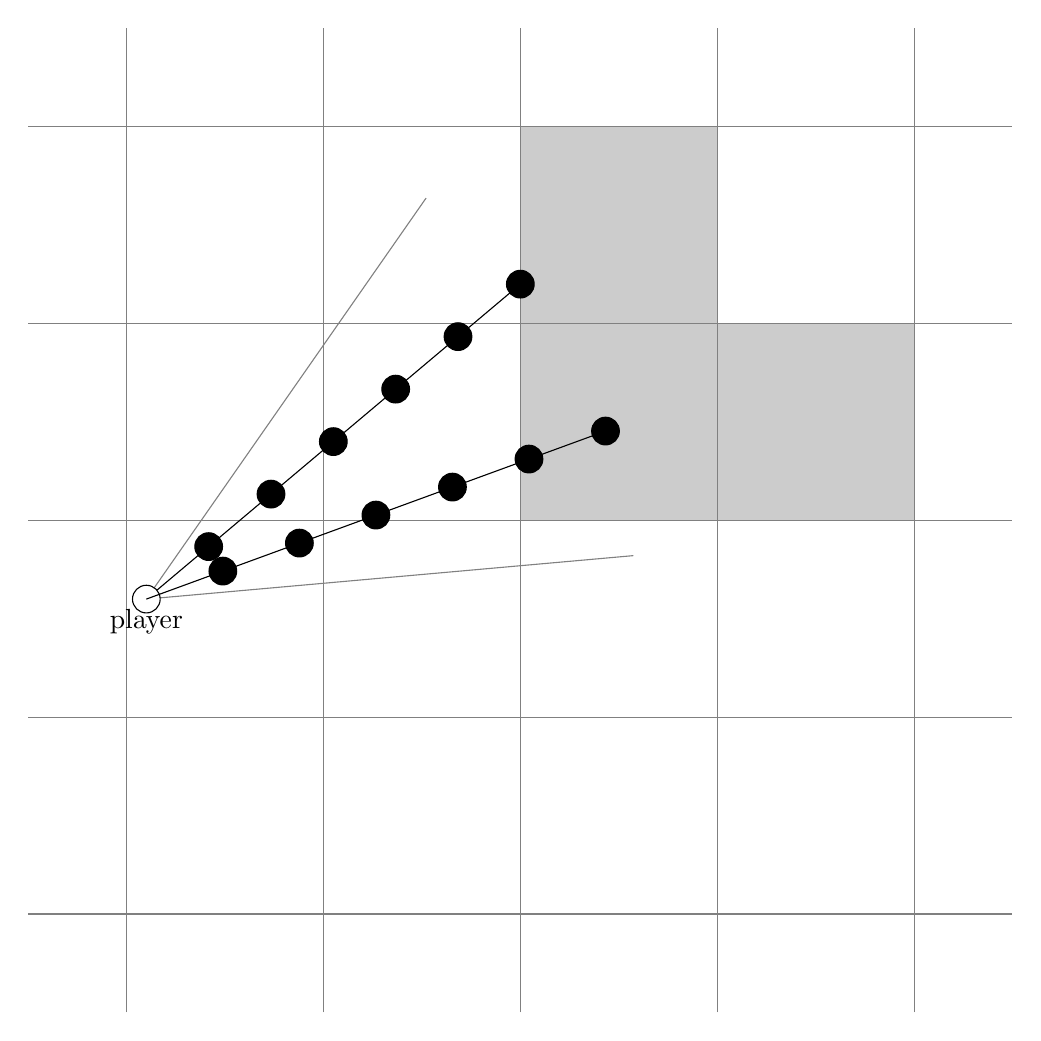
\begin{tikzpicture}[scale=2.5]


\coordinate(player) at (2.1,3.6) {};
\coordinate(intercept) at (4,5.2) {};

%FOV
\coordinate[](left_edge) at ($(player)!1!15:(intercept)$);
\coordinate[](right_edge) at ($(player)!1!325:(intercept)$);
\draw[draw=gray] (player) -> (left_edge) ;
\draw[draw=gray] (player) -> (right_edge) ;




\fill[black!20!white, draw=black] (4,5) rectangle (5,6);
\fill[black!20!white, draw=black] (4,4) rectangle (5,5);
\fill[black!20!white, draw=black] (5,4) rectangle (6,5);

%grid
% vertical lines
\draw[draw=gray] (2,1.5) -- (2,6.5) ;
\draw[draw=gray] (3,1.5) -- (3,6.5) ;
\draw[draw=gray] (4,1.5) -- (4,6.5) ;
\draw[draw=gray] (5,1.5) -- (5,6.5) ;
\draw[draw=gray] (6,1.5) -- (6,6.5) ;

% horizontal lines
\draw[draw=gray] (1.5,2) -- (6.5,2) ;
\draw[draw=gray] (1.5,3) -- (6.5,3) ;
\draw[draw=gray] (1.5,4) -- (6.5,4) ;
\draw[draw=gray] (1.5,5) -- (6.5,5) ;
\draw[draw=gray] (1.5,6) -- (6.5,6) ;
%\draw[] 

\draw[draw=black] (player) -- (intercept) ;
\fill[draw=black, fill=white] (player) circle (2pt);
\fill[draw=black] (intercept) circle (2pt);

\draw(player)node[below]{player};



\fill[draw=black] ( $ (player)!5/6!(intercept) $ ) circle (2pt);
\fill[draw=black] ( $ (player)!4/6!(intercept) $ ) circle (2pt);
\fill[draw=black] ( $ (player)!3/6!(intercept) $ ) circle (2pt);
\fill[draw=black] ( $ (player)!2/6!(intercept) $ ) circle (2pt);
\fill[draw=black] ( $ (player)!1/6!(intercept) $ ) circle (2pt);


\coordinate[](missed_intercept) at ($(player)!1!340:(intercept)$);
\draw[draw=black] (player) -- (missed_intercept) ;
\fill[draw=black] (missed_intercept) circle (2pt);
\fill[draw=black] ( $ (player)!5/6!(missed_intercept) $ ) circle (2pt);
\fill[draw=black] ( $ (player)!4/6!(missed_intercept) $ ) circle (2pt);
\fill[draw=black] ( $ (player)!3/6!(missed_intercept) $ ) circle (2pt);
\fill[draw=black] ( $ (player)!2/6!(missed_intercept) $ ) circle (2pt);
\fill[draw=black] ( $ (player)!1/6!(missed_intercept) $ ) circle (2pt);

\end{tikzpicture}
\end{document}
